\documentclass[../main.tex]{subfiles}

\begin{document}

\section{Estabilidad del equilibrio en placa}



Esta parte es importante para la seguridad estructural. Es posible ver lo que 
se realiza en la siguiente imagen:

\begin{figure}[htpb]
  \centering
  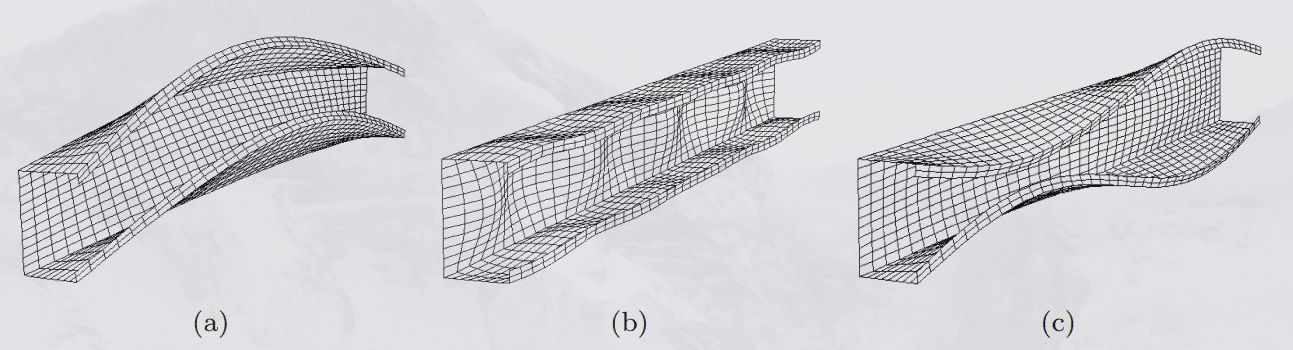
\includegraphics[width=0.8\textwidth]{../images/20210517/pandeo_local}
  \caption{Ejemplos de pandeo localizado.}
  \label{fig:pandeo_local}
\end{figure}

Estos problemas son más preponderantes son en los perfiles delgados, que serán
perfiles no compactos.

\subsection{Pandeo en placas planas}

Podemos tener dos tipos de pandeos: el pandeo precrítico y el pandeo poscrítico.
El \textbf{pandeo precrítico} puede ser elástico o inelástico, mientras que el
\textbf{pandeo poscrítico} es siempre inelástico.

Existen soluciones gráficas y formulas simples que permite resolver las ecuaciones
diferenciales para la resolución de este tipo de problemas, que en principio se
como:

\begin{align*}
  F_{ki} = k * \frac{\pi^{2}*E}{12*(1-\mu)}*\frac{1}{(b / t)^{2}}
.\end{align*}

Donde el valor de $k$ depende de como esta apoyada la columna de los lados no
cargados, que puede ser obtenido de la \Cref{fig:valork}

\begin{figure}[htpb]
  \centering
  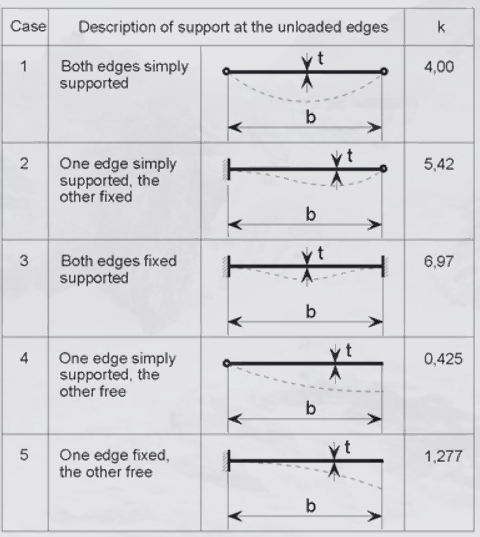
\includegraphics[width=0.8\textwidth]{../images/20210517/valork}
  \caption{Valores de K}
  \label{fig:valork}
\end{figure}

Cabe notar que estos valores dependerá de las condiciones de apoyo perpendicular
a la fuerza.

\subsubsection{Pandeo precrítico elástico}

Utilizando la formula ya dada, se puede encontrar el valor de $k_1$ para encontrar
el corte critico como se desarrolla:

\begin{align*}
  \tau_{ki} = k * \frac{\pi^{2}*E}{12*(1-\mu)}*\frac{1}{(b / t)^{2}}
.\end{align*}


\begin{align*}
  k_1 &= 5.34 + \frac{4}{\alpha²} \hspace{0.25cm} \xrightarrow{\hspace*{0.5cm}} \hspace{0.1cm} \alpha \geq 1  \\[5pt]
  k_1 &= 4 + \frac{5.34}{\alpha²} \hspace{0.25cm} \xrightarrow{\hspace*{0.5cm}} \hspace{0.1cm} \alpha \leq 1 
.\end{align*}

Donde el valor de $\alpha$ es  $a/h$. Los problemas dados por el corte se
encuentran principalmente cerca del apoyo, donde los esfuerzos son máximos.

La forma de poder mejorar la situación es mediante la utilización de
\textbf{rigidizadores}, que nos permiten reducir la distancia $a$. 

\subsubsection{Pandeo precrítico inelástico}

Se puede hacer mediante la fórmula de Basler, que es:

\begin{align*}
  \tau_{cr} = \sqrt{\tau_{pr}*\tau_{ki}} 
.\end{align*}

\subsubsection{Combinación de tensiones}

Se nos puede dar la situación donde se tengan tanto tensiones normales y 
tangenciales. Esto es necesario considerar una formula mucho más compleja que
considera las tensiones reales actuantes, tensiones críticas sin sobreposición
y relaciones de tensiones, aunque es posible hacerlo mediante el reglamento
de forma simplificada.

\subsection{Pandeo poscrítico}

Es una sobretensión que es posible aprovechar. Se da cuando, luego del pandeo 
dado que luego del pandeo la distribución de tensiones se da de forma distinta,
bajando en el medio y aumentando en los costados, incluso superando la tensión
crítica de pandeo, que se da porque los bordes son indesplazables y permiten
entonces tomar más carga. Esto se ve en \Cref{poscrtitico}.

\begin{figure}[htpb]
  \centering
  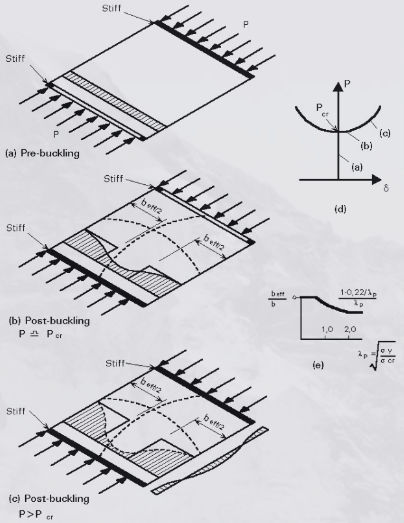
\includegraphics[width=0.8\textwidth]{../images/20210517/poscritico}
  \caption{Pandeo poscrítico.}
  \label{fig:poscritico}
\end{figure}

Esto se da mediante el concepto de \textbf{ancho efectivo}, que es menor al
ancho real, que nos da el valor de la carga crítica considerando la 
sobreresistencia.


\end{document}
